\chapter{2006:Jon Kleinberg}
\label{chap:kleinberg}
\begin{center}
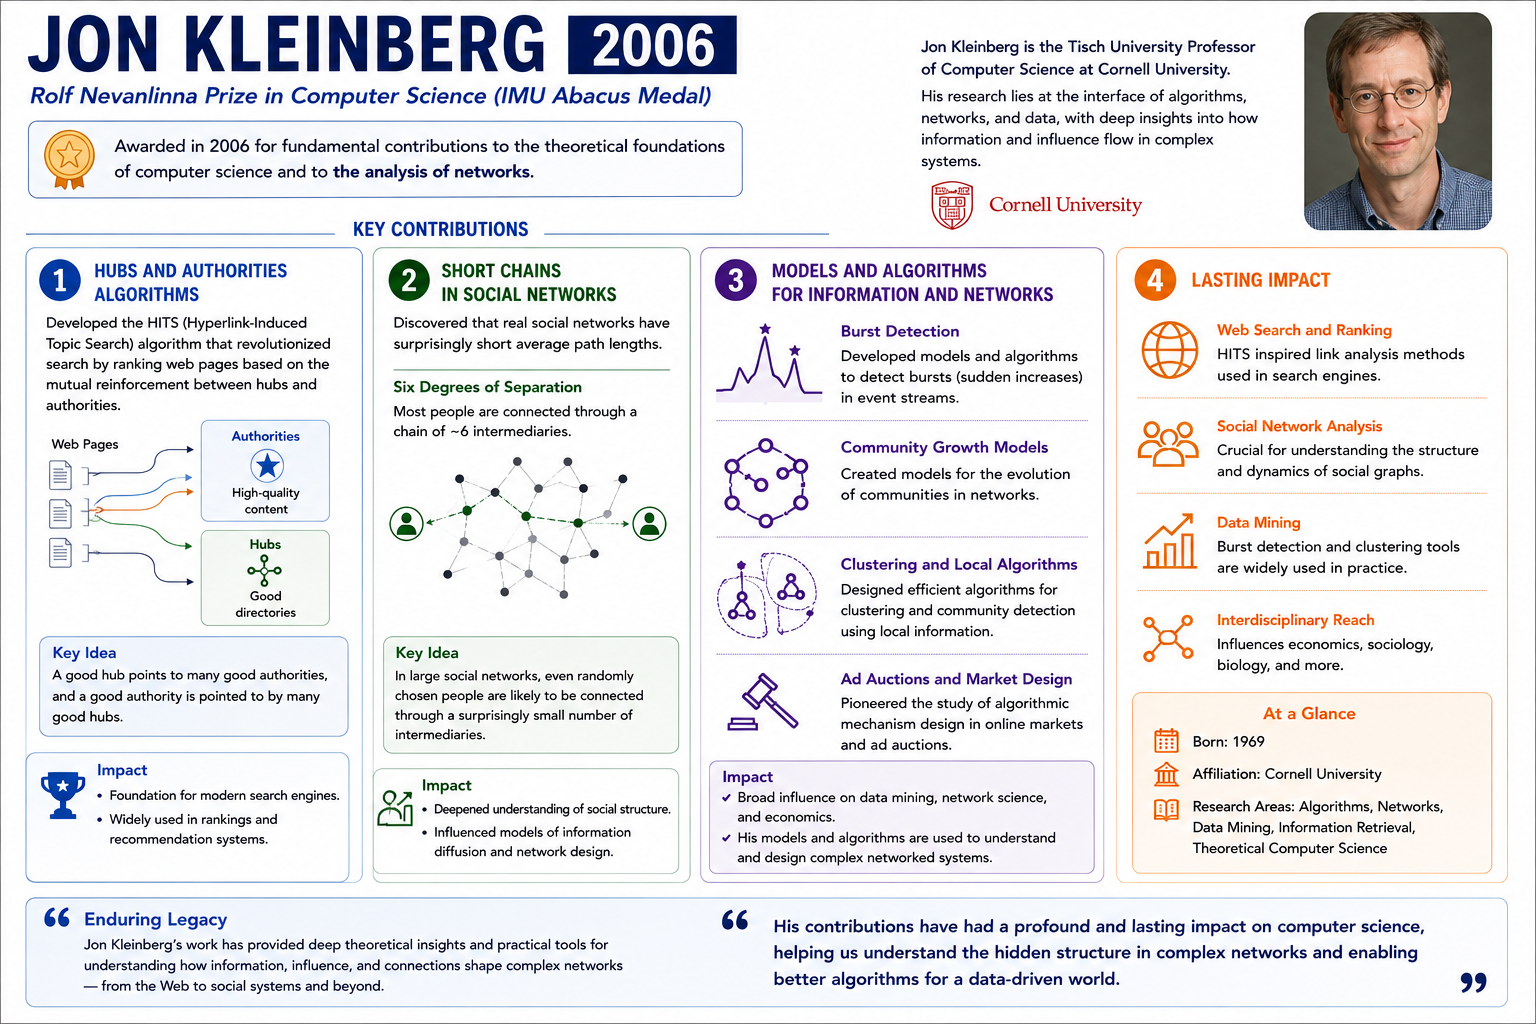
\includegraphics[width=\textwidth]{infographics/abacus7.png}
\end{center}
\targetchapterspacing
\index{Kleinberg, Jon}
\booknote{The central habit in this chapter is to state what local information an algorithm may use and what global question it must answer---and then to name the reinforcement rule whose equilibrium the answer represents.}

\section{An Opening Story: A Recipe Site Where Popularity Is Circular}
Maya runs a small cooking site with four pages. Page A holds a famous lasagna recipe; page B, a weeknight-dinner blog, links to A; page C, a family recipe box, links to B and A; page D, a kitchen forum, links to C. Nobody links to D.

Which page answers ``lasagna''? Count incoming links: A has two, B and C have one, D has none. Ask which is most \emph{trusted} and the reasoning turns circular: A is trusted because good pages point to it, B because C points to it, C because D points to it, D because \ldots nothing. Popularity defined by popularity has no answer until we agree on a rule that breaks the circle.

\section{The Problem}
Network data arrives locally: a search engine sees millions of pages and the links among them; a person reaching a stranger sees only their own friends; a log shows one event at a time. Yet the questions worth asking are global: which pages are authoritative? Can someone reach a distant person using only nearby contacts? Is an hour of frantic activity a real story or ordinary noise?

A single local observation carries almost no information; the answer lives in the whole pattern. The difficulty is \emph{aggregation}. Three problems make this concrete:
\begin{itemize}
\item \textbf{Ranking.} Given the web's links, rank pages so authoritative ones rise to the top.
\item \textbf{Navigation.} Given a network with long-range shortcuts, reach a distant target using only local information.
\item \textbf{Burst detection.} Given a stream of timestamped events, decide when the rate genuinely rises and where bursts begin and end.
\end{itemize}
Each is easy to state and easy to get wrong: ranking is gameable, navigation can be blocked by information never seen, and bursts hide inside random variation.

\section{The World Before}
Early search engines matched query words against page text. Simple---and a standing invitation to cheat: a page repeating ``lasagna recipe'' twenty times outranked a better page using the phrase once. Keyword-stuffed pages became the norm; raw text was trivial to game.

Counting incoming links was the natural fix: more pages pointing at you meant more people found you useful. Harder to fake with one page, but not with a thousand---a \emph{link farm} is a cluster of pages built only to point at one target. Counting also hid the circularity of the recipe puzzle: a page is popular partly because \emph{popular} pages link to it.

Social networks had a folklore theorem: Milgram's letter experiments suggested a small diameter, about six handoffs between any two people, so navigation must be easy. But a person can only hand a letter to someone they know. Small diameter says a short path \emph{exists}; it says nothing about whether someone who sees only their own acquaintances can \emph{find} it. The inference---short paths imply easy navigation---is not merely unproven; it is false.

Bursts had a statistical description, but no algorithm for finding where a rate changes; eleven messages in ten minutes could be a burst or ordinary luck. Two ideas were missing: an \emph{explicit model of mutual reinforcement}, turning circular importance into a computable fixed point, and an \emph{explicit model of the information a local navigator has}, separating ``a short path exists'' from ``a local rule can find it.'' Kleinberg's 2006 Nevanlinna Prize recognized precise answers to all three.

\section{The New Idea}
\subsection{HITS: two roles, one fixed point}
An \emph{authority} is worth reading; a \emph{hub} is worth following. They reinforce each other: good authorities are linked by good hubs, and good hubs link to good authorities.

Break the circle by iteration. Start every score at $1$, then alternate:
\begin{itemize}
\item \textbf{Authority update:} new authority $=$ sum of the hub scores of the pages linking to it.
\item \textbf{Hub update:} new hub $=$ sum of the authority scores of the pages it links to.
\end{itemize}
Rescale after each round. The mutual definition becomes concrete arithmetic that settles down. In matrix language,
\[
a\leftarrow A^{\mathsf T}h,\qquad h\leftarrow Aa,
\]
and the stable scores are the principal singular vectors of the adjacency matrix $A$.

\subsection{The small-world model: what a local navigator can use}
Lay the network on a two-dimensional grid. Each person knows their grid neighbors and a few \emph{shortcuts}---long-range contacts. The navigator's rule is greedy and myopic: move to the contact closest to the target; no one sees the map.

Suppose node $u$ links to node $v$ with probability proportional to $d(u,v)^{-r}$. The answer is sharp:
\begin{itemize}
\item $r=2$: polylog expected steps;
\item $r<2$: too-uniform shortcuts---polynomial time;
\item $r>2$: too-local shortcuts---polynomial time.
\end{itemize}
The $2$ is the grid's dimension. From distance $\delta$ to the target, the useful jumps land in the \emph{halving ball}---nodes within $\delta/2$ of the target---about $\delta^{2}$ of them, each reached with probability about $1/\delta^{2}$. A useful jump has comparable probability at every scale, so $\log_2 n$ halvings reach the target.

\subsection{Bursts: separating a baseline from a self-exciting process}
A burst is a stretch in which events arrive faster than the baseline rate. Kleinberg's model uses hidden states: a normal state at rate $\lambda_0$ and a burst state at rate $\lambda_1>\lambda_0$. Assigning each event to a state while explaining the observed waiting times and paying a penalty per switch turns a burst into an \emph{inferred hidden structure} rather than a claim that each event directly causes the next.

\subsection{The conceptual shift}
All three models make explicit what information the algorithm may use and what rule converts it into an answer. The conclusions are precise and surprising: \emph{local connectivity can generate useful global signals, but only when the definition of relevance is explicit; and small diameter does not imply navigability.}

\section{How It Works: Worked Examples}
\subsection{Example 1: HITS by hand on four pages}
Maya's site as a directed graph: $B\to A$, $C\to A$, $C\to B$, $D\to C$. Start all scores at $1$.

Round 1, authority ($a_j=$ sum of hub scores of pages linking to $j$):
\[
a_A=h_B+h_C=2,\qquad a_B=h_C=1,\qquad a_C=h_D=1,\qquad a_D=0.
\]
Round 1, hub ($h_i=$ sum of authority scores of pages $i$ links to):
\[
h_A=0,\qquad h_B=a_A=2,\qquad h_C=a_A+a_B=3,\qquad h_D=a_C=1.
\]
Round 2, authority:
\[
a_A=h_B+h_C=2+3=5,\qquad a_B=h_C=3,\qquad a_C=h_D=1,\qquad a_D=0.
\]
Round 2, hub:
\[
h_A=0,\qquad h_B=a_A=5,\qquad h_C=a_A+a_B=5+3=8,\qquad h_D=a_C=1.
\]
Collect the two rounds: authority $(2,1,1,0)\to(5,3,1,0)$, hub $(0,2,3,1)\to(0,5,8,1)$. A rises as the dominant authority, C as the dominant hub. Renormalizing after each round---dividing by the length of each score vector---keeps the iteration convergent without changing which page is largest. These scores are the \emph{equilibrium of this rule}, not an objective fact about the pages.

\subsection{Example 2: greedy routing on a 4 by 4 grid}
Draw a $4\times4$ grid, target at $(4,4)$, navigator at $(1,1)$; without shortcuts the trip takes $6$ steps.

Give $(1,1)$ a shortcut to $(3,3)$. Greedy compares options: $(1,2)$ is $5$ from the target, $(2,1)$ is $5$, the shortcut endpoint is $2$. It jumps, then $(3,3)\to(3,4)\to(4,4)$: three steps, and the jump cut the remaining distance from $6$ to $2$---roughly in half.

How should shortcuts be distributed? From the corner $(1,1)$ the grid has two nodes at distance $1$, three at $2$, four at $3$, three at $4$, two at $5$, one at $6$. Under $r=2$ (probability proportional to $1/d^2$):
\begin{center}
\begin{tabular}{lcccccc}
\toprule
distance $d$ & 1 & 2 & 3 & 4 & 5 & 6 \\
\midrule
chance & $57\%$ & $21\%$ & $13\%$ & $5\%$ & $2\%$ & $0.8\%$ \\
\bottomrule
\end{tabular}
\end{center}
Short jumps dominate; under a uniform law ($r=0$) every distance is equally likely at about $6.7\%$, so no scale can be counted on. The contrast is decisive at scale $n$: the halving ball holds about $\delta^{2}$ nodes, each reached with probability about $1/\delta^{2}$, so a useful jump has comparable chance at every scale and $\log_2 n$ halvings reach the target. Under $r<2$ the longest links dominate and the halving chance collapses; under $r>2$ shortcuts almost never reach half the gap. Both force polynomial time.

\section{The Mathematics in Brief}
\textbf{HITS.} The iteration
\[
a\leftarrow A^{\mathsf T}h,\qquad h\leftarrow Aa
\]
with normalization is power iteration for the symmetric matrices $A^{\mathsf T}A$ and $AA^{\mathsf T}$, converging to the principal singular-vector pair of $A$. \emph{Why:} substituting gives $a\leftarrow A^{\mathsf T}Aa$, and repeated multiplication by a symmetric matrix amplifies the largest-eigenvalue direction while shrinking all others.

\textbf{Small-world navigation.} Shortcuts follow
\[
\PP(u\text{ links to }v)\propto d(u,v)^{-r}.
\]
On an $n\times n$ grid, greedy routing takes $O((\log n)^2)$ expected steps when $r=2$ and $\Omega(n^{\beta})$ for a constant $\beta>0$ when $r\ne2$. \emph{Why:} under $r=2$ the normalization sum is $\Theta(\log n)$, so the halving ball is hit with probability $\Theta(1/\log n)$ per shortcut; under $r<2$ the halving chance is $\Theta((\delta/n)^{2-r})$; under $r>2$ shortcuts never reach the ball. The exponent must equal the dimension.

\textbf{Bursts.} Waiting times are exponential at rate $\lambda_0$ in the normal state and $\lambda_1>\lambda_0$ in the burst state; the model picks the assignment of events to states that best explains the observed waits, minus a penalty per switch. \emph{Why:} a constant-rate model predicts long runs of very short waits to be exponentially unlikely, so when they occur a state switch is the parsimonious explanation; the penalty stops a new burst being declared around every event.

\textbf{The distinction.} A centralized algorithm knows the whole graph; a navigator sees only its position and contacts. ``There is a short path'' and ``a local rule can find it'' are different statements, and the small-world theorem draws the line between them.

\section{Limits and Modern Views}
The HITS equilibrium is not a neutral measure. A tightly connected community can dominate without being globally authoritative, and a feedback loop can lock in an early accident: top-ranked pages attract attention, attention creates links, links raise the rank \cite{kleinberg-hits}. A link is not a causal statement: two pages may link because they share an audience, a platform may recommend both, and friendship and purchase may share a hidden cause. Rankings amplify these hidden causes, so modern work asks causal questions alongside graph questions \cite{kleinberg-smallworld}.

Models are static while networks move, so a static eigenvector lags the system it summarizes; popularity attracts links partly because it is already popularity. Strategic actors game whatever signal is scored---link farms, coordinated bots, engineered cascades---so the evidence is adversarial \cite{kleinberg-bursts}. Rankings encode past inequalities, attention measurements touch privacy, and an engagement-optimal ranking can worsen the decision it supports; fairness-aware and privacy-preserving models now share the agenda.

Kleinberg's style survives these harder questions: name the mechanism, derive a testable prediction, then check which parts survive contact with data. The model is a hypothesis to test, not reality itself.

\section{Exercises and Self-Study Guide}
\begin{enumerate}[label=\textbf{E\arabic*.}]
\item Run one more HITS round on the worked example from $a=(5,3,1,0)$, $h=(0,5,8,1)$. Confirm $A$ stays the top authority and $C$ the top hub.
\hint{Authority of a page is the sum of the hub scores of pages linking to it; hub is the sum of the authority scores of the pages it links to.}
\item On the three-page graph $A\to B$, $A\to C$, $B\to C$, compute two HITS rounds from all-ones scores. Which page becomes the top authority, and which the top hub?
\hint{$a_A=0$ because nothing links to $A$; $C$'s authority and $A$'s hub score grow fastest.}
\item On a $3\times3$ grid, place a shortcut from $(2,2)$ to $(1,1)$ and run greedy routing to target $(1,1)$ from $(2,2)$ and from $(1,3)$. When does the shortcut help, and when is it invisible?
\hint{Greedy moves to the contact closest to the target; a shortcut is usable only from its source node.}
\item Two streams of twenty events each: $S$ has one event every 100 minutes; $T$ has nineteen events in the first 90 minutes, then silence. Same average rate. Which is a burst, and how does a model detect it?
\hint{Compare inter-arrival times: $S$ has waits near 100 minutes, $T$ has many tiny waits followed by one huge one.}
\item Describe a confounding variable that could make friendship links look as though they cause purchases.
\hint{A shared experience---a new TV show, a holiday, a company policy---can create both the friendship and the purchase.}
\item Remove the link $D\to C$ and rerun HITS for two rounds. Does $A$ remain the top authority? Propose a simple stability test for a ranking when links change.
\hint{Rerun with the link deleted and compare the ordering of the top pages before and after.}
\item On the $4\times4$ grid, put a shortcut from $(1,2)$ to $(4,4)$ and route from $(1,1)$ to $(4,4)$. With full knowledge the shortest path is $(1,1)\to(1,2)\to(4,4)$: two steps. Simulate greedy, breaking ties toward the larger row number. How many steps, and why does it miss the shortcut?
\hint{Greedy sees a shortcut only when standing at its source; the tie-break at $(1,1)$ decides whether the walk ever reaches $(1,2)$.}
\end{enumerate}

\booknote{A final exercise in judgment: whenever a ranking is published or a path is followed, name the reinforcement rule that produced the score and the local information the navigator was allowed to see. A number that cannot be traced to a stated rule is not a finding; it is a guess wearing notation.}
\clearpage
